\section{Project Stage}
\subsection{System Architecture}

\begin{figure}[H]
	\centering
	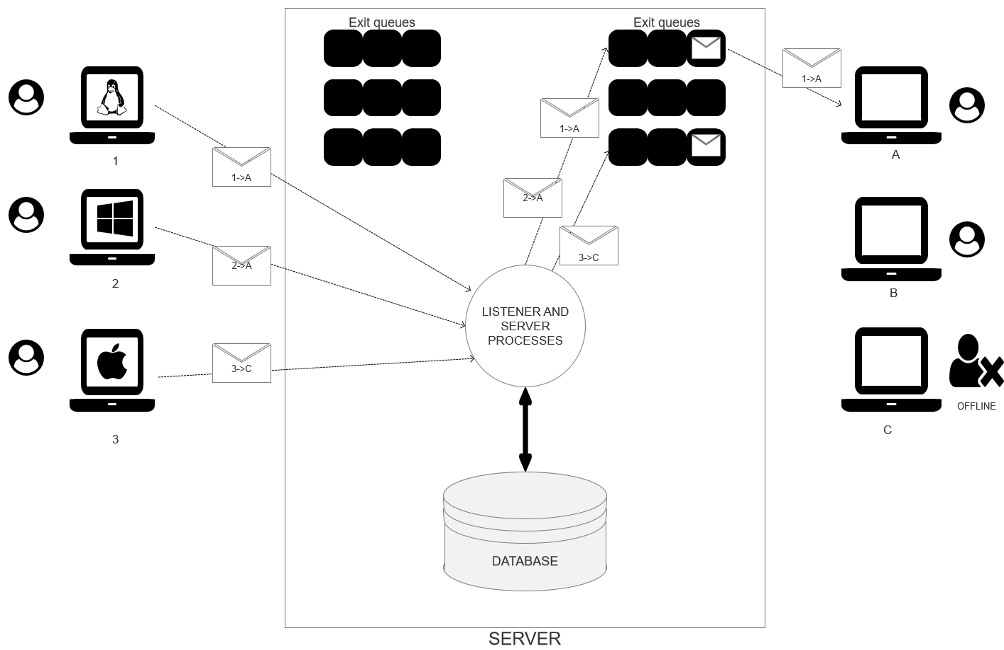
\includegraphics[width=\textwidth]{img/systemArchitecture.png}  
\end{figure}

As shown in the previous picture, the application is based on a client-server architecture, in which each client, in order to send a \textbf{message} to a \textbf{user}, contacts the main server which is in charge of determining receiver’s physical address and forward the \textbf{message} if it is online.
In the image some typical scenarios are represented to help better understand how \textit{Unisup} works. In particular:
\begin{enumerate}
	\item The message 1 $\xrightarrow{}$ A is sent from the client 1 destined to the client A:  it arrives at the main server that pushes it into the corresponding queue. The client A is online and there is no message to consume on the queue, so it is immediately forwarded.
	\item The message 2 $\xrightarrow{}$ A is sent from the client 2 destined to the client A:  as the previous one, it is pushed into A’s queue but this time the channel is busy. The message will be forwarded as soon as the channel comes idle again.
	\item The message 3 $\xrightarrow{}$ C is sent from client 3 destined to C: again, it is pushed on the correct queue. C is offline, so the message is not forwarded; it will be delivered as soon as C turns online again.
\end{enumerate}	
The OS picture inside clients means that the system works on every OS.
Eventually, the database icon has been added since it is required for mapping clients’ addresses and store chat histories. 


\subsection{Clients}
\subsubsection{Role of the Client}
\subsubsection{Technologies}

\subsection{The Server}
\subsubsection{Role of the Server}
\subsubsection{Persistent Data Storing}
\subsubsection{Queueing}

\subsection{Synchronization Management}
\subsubsection{Client-Side}
\subsubsection{Server-Side}

\subsection{Sequence UML Diagrams}